\documentclass[12pt]{article}
\newtheorem{prob}{Problema}
\newtheorem{defi}{Definición}
\newtheorem{ejem}{Ejemplo}
\newtheorem{sol}{Solución}
%Paquetes a utilizarse
\usepackage[width=7in, height=9.5in, top=0.75in, papersize={8.5in,11in}]{geometry}
\usepackage[spanish]{babel} 
\decimalpoint
\usepackage[utf8]{inputenc}
\usepackage{bbding}
\usepackage[colorlinks = true, linkcolor = blue, urlcolor = BlueViolet, citecolor = OliveGreen]{hyperref}
\usepackage{graphicx}
\usepackage{amssymb,amsthm,amsmath}
\usepackage{enumerate}
\usepackage{array,multicol,multirow}
\usepackage{xcolor}
\usepackage{fancybox,tcolorbox}
\usepackage{caption,subcaption,float,tabularx}
\usepackage{enumitem}

\theoremstyle{definition}
\newtheorem{corolario}{Corolario}
\newtheorem{lema}[corolario]{Lema}
\newtheorem{proposicion}[corolario]{Proposición}
\newtheorem{teorema}[corolario]{Teorema}
\newtheorem{propiedad}[corolario]{Propiedad}
\newtheorem*{observacion}{Observación}
\newtheorem{definicion}{Definición}
\newtheorem*{demostracion}{Demostración}
\newtheorem{ejemplo}{Ejemplo}
\newtheorem{problema}{Problema}
\newtheorem*{solucion}{Solución}
\newtheorem{ejercicio}{\PencilRightDown \  Ejercicio}
\newtheorem{step}{Paso}
\newtheorem{credito}{Crédito}

\usepackage{tikz}
\usetikzlibrary{arrows.meta,babel,calc,positioning}

\renewcommand{\arraystretch}{1.5}
\providecommand{\abs}[1]{\lvert#1\rvert}
\providecommand{\norm}[1]{\lVert#1\rVert}

\renewcommand{\tabularxcolumn}[1]{m{#1}}
\newcommand{\Evaluacion}[4]{
\setcounter{ejercicio}{0}
\noindent\begin{tabular}{lcr}
	\includegraphics[height=3cm]{Logos/logo-UES.png}\hspace{2.5em}
	&
	\includegraphics[height=2.75cm]{Logos/logo-PJT.png}
	& 
	\hspace{2.5em}\includegraphics[height=2.75cm]{Logos/logo-MINEDUCYT.png}
\end{tabular}

\hfill

\begin{center}
    
    UNIVERSIDAD DE EL SALVADOR
    \\PROGRAMA JÓVENES TALENTO
    \\FDTC 2022
    \\#2
    \\Nivel Olímpico C de Matemáticas

\end{center}

\begin{center}
    #1
\end{center}

%\textbf{Nombre}: \enspace\hrulefill

#3

\input{#4}
\newpage
}

\newtheorem{obs}{Observación}

%\usepackage[margin=2.5cm]{geometry}
%\usepackage{wasysym}
%\usepackage{stmaryrd,textcomp}
%\usepackage{pgf,tikz}
%\usetikzlibrary{arrows}

\parskip = 2mm   %%%% genera un espacio de X mm entre lo párrafos
\parindent = 3mm
\usepackage{multicol}
\usepackage{iwona}

\newcommand{\tema}{Principios fundamentales}
\newcommand{\fecha}{Miércoles, 30 de noviembre de 2022}
\newcommand{\sesion}{Sesión 2}

\begin{document}
%\thispagestyle{empty}
%\newpage
\thispagestyle{empty}

\begin{figure}[h] 
	\begin{minipage}[b]{0.26\textwidth}
		\begin{center}
			
\includegraphics[height=3cm]{Logos/UES.png}
			\par\end{center}
	\end{minipage} 
	\begin{minipage}[b]{0.46\textwidth}
		\begin{center}
			UNIVERSIDAD DE EL SALVADOR\\ [0.1cm]
			PROGRAMA JÓVENES TALENTO\\ [0.1cm]
	        FDTC 2022\\ [0.1cm]
                NIVEL 5\\ [0.1cm]
			COMBINATORIA 
			\par\end{center}
	\end{minipage} 
	\begin{minipage}[b]{0.05\textwidth}
		\begin{center}
			
\includegraphics[height=2cm]{Logos/LOGO PJT.png}
			\par\end{center}
	\end{minipage}
\end{figure}

\begin{center}
    \begin{tabular}{p{4.5cm} p{7cm} p{4.5cm}}
        \tema & \centering\fecha & \hfill\sesion
    \end{tabular}
\end{center}
\section{Ejercicios de repaso}
\begin{ejercicio}
    Sean los conjuntos $A=\left\{-\beta,2\right\}$ y $B=\left\{\beta^2-7,\beta+1,3\right\}$. Si $A\subseteq B$, ¿qué número real debe ser $\beta$?
\end{ejercicio}

\begin{ejercicio}
    Si $X$ es el conjunto de todos los enteros positivos impares menores que $70$, ¿cuál es el número de elementos en $X$?
\end{ejercicio}

\begin{ejercicio}
    ¿Cuántos elementos hay en el conjunto $X=\left\{16,18,20,\ldots,96,98,100\right\}$?
\end{ejercicio}

\begin{ejercicio}
     Si $\mathbb{Z}$ denota al conjunto de los números enteros y sea $\Omega$ el conjunto
    \[\Omega=\left\{8,\frac{2}{3}+\frac{3}{9},\sqrt[3]{8},\frac{54}{6},-6,0,2+\sqrt{16},-\frac{\sqrt{36}}{4},1^{-2},\frac{3^4-2^4}{3^2+2^2}\right\},\]
    ¿cuántos elementos hay en $\mathbb{Z}\cap \Omega$?
\end{ejercicio}

\begin{ejercicio}
     Si $X=\left\{2,3,4\right\}$ e $Y=\left\{3,4,8,9,11,14\right\}$, ¿cuántos conjuntos $Z$ satisfacen que
    \[(X-Y)\cup Z=Z,\;\;\;\; (X\cup Y)\cap Z=Z\text{?}\]
\end{ejercicio}

\begin{ejercicio}
    Sea $N$ un subconjunto del conjunto
    \[M=\left\{1,2,3,\ldots,k\right\}\]
    tales que $1$ y $2$ son elementos que están en $N$ pero que $3$ y $4$ no están en $N$. Si hay un total de $128$ de tales subcojuntos $N$, ¿cuánto  vale $k$?
\end{ejercicio}
\section{Principios fundamentales en el conteo}
Imagínate por un momento que vas de compras en algún día tranquilo de la semana. Seleccionas un buen par de jeans y decides pagar con tu tarjeta de crédito (o con la de sus padres). Pero de repente te das cuenta de que no puedes recordar tu pin. ¡Qué tragedia! Ahora todo lo que se te ocurre es hacer una lista de todas las combinaciones posibles para descubrir tu pin. \textit{¿Cuántas combinaciones posibles puedes hacer?} La respuesta a esta pregunta es \textit{difícil} si seguimos enumerando cada combinación posible y contando. En situaciones como estas, el principio fundamental del conteo o el principio de multiplicación viene a nuestro rescate. Y en otras situaciones con más restricciones es pertinente usar el conocido principio de la suma. En esta lección vamos a estudianr ambos resultados y haremos hincapié en las aplicaciones así como en su diferenciación.
\subsection{Principio de la multiplicación}
\begin{definicion}
    El principio fundamental de conteo o principio de la multiplicación es una regla que se usa para contar el número total de resultados posibles en una situación. Establece que si hay $n$ formas de hacer algo y $m$ formas de hacer otra cosa después de eso, entonces hay $n\times m$ formas de realizar ambas acciones. En otras palabras, al elegir una opción para $n$ y una opción para $m$, hay $n \times m$ formas diferentes de realizar ambas acciones.
\end{definicion}

\begin{ejemplo}
    En el armario de Brenda hay $4$ pantalones diferentes, $9$ camisas diferentes y $n$ chaquetas diferentes. Si la cantidad de combinaciones de pantalones, camisas y chaquetas que Brenda puede elegir es $252$, ¿cuántas chaquetas diferentes tiene?
\end{ejemplo}

\begin{solucion}
    Para cada una de las $n$ chaquetas diferentes, hay $4$ pantalones diferentes y $9$ camisas diferentes para elegir. Así, el número total de combinaciones es de $4\times 9 \times n$ y lo cual
    \begin{eqnarray*}
        4\times 9 \times n&=&252\\
        n&=&7
    \end{eqnarray*}
    Así, Brenda tiene $7$ chaquetas diferentes.
\end{solucion}

\begin{ejemplo}
    ¿Cuántos divisores positivos tiene $2000=2^4\cdot 5^3$?
\end{ejemplo}

\begin{solucion}
    Cualquier divisor del número $2000$ debe tener la forma $2^m\times 5^n$, donde $0\leq m\leq 4$ y $0\leq n\leq 3$. En consecuencia, hay $5$ posibilidades para $m$ y $3$ posibilidades para $n$. Por tanto, hay
    \[5\times 4=20\]
    divisores positivos de $2000$ en total.
\end{solucion}

\begin{ejemplo}
    ¿De cuántas maneras se pueden elegir un presidente y un vicepresidente de $25$ candidatos?
\end{ejemplo}

\begin{solucion}
De los $25$ candidatos, hay $25$ formas posibles de elegir un presidente. Después de elegir al presidente, quedan $24$ candidatos para elegir un vicepresidente. Por el principio de la multiplicación tenemos entonces que hay
\[25\times 24=600\]
maneras de elegir al presidente y al vicepresidente.
\end{solucion}

\begin{ejemplo}
    Erick fue a la tienda después de la escuela para recoger una jarra de leche, una barra de pan, una docena de huevos y un paquete de galletas. La leche viene en variedades de $1\%$, $2\%$ y $3,25\%$. El pan viene en blanco y $100\%$ integral. Los huevos vienen en paquetes de docenas de varios tamaños: pequeños, medianos, grandes y jumbo. Las galletas vienen en tres sabores diferentes. ¿De cuántas maneras diferentes puede Erick llevar a casa los elementos de su lista?
\end{ejemplo}

\begin{solucion}
Usamos la propiedad de multiplicación de contar, ya que Erick está comprando uno de cada artículo. Tiene $3$ opciones de leche, $2$ de pan, $4$ de huevos y $3$ de galletas, así que tiene $3\times 2 \times 4 \times 3=72$ diferentes maneras de llevar a casa los elementos de su lista.
\end{solucion}

\begin{ejemplo}
Si cuenta las formas de subir 3 escalones encontrará que hay 4 formas de subir 3 escalones. Imagine que las piernas de la persona son tan largas que tiene la capacidad de subir 11 escalones a la vez. Además, a la persona solo se le permite subir hacia arriba. Encontrar el número de formas en que puedes subir 11 escalones. \textbf{Bonificación}: Generalice esto para $n$ pasos.
\end{ejemplo}

\begin{solucion}
Aquí, hay $11$ escalones. Ahora, pisar cualquiera de los primeros $10$ escalones no es obligatorio, pero es obligatorio para el $11^\circ$ Escalón, porque es donde tenemos que subir. Entonces, hay $2$ opciones para los primeros $10$ escalones, pero solo $1$ para el $1$. Por lo tanto, según la regla del producto, el número de formas de subir a la escalera $11$ es:
\[2\times 2\times 2\times 2\times 2\times 2\times 2\times 2\times 2\times 2\times 1=2^{10}=1024\;. \]
La persona tiene que subir el escalón $n$-ésimo obligatoriamente. Pero la persona en los primeros $n-1$ escalones lo pisa o no lo pisa. Por lo tanto, hay $2$ posibilidades para cada paso de los $n-1$ escalones. Entonces, por regla de la multiplicación, el total de formas es \[\underbrace{2\times 2 \ldots \times 2}_{n-1\;\text{veces}}\times 1=2^{n-1}\]
y si $n=11$, nuestra resolución es consistente.
\end{solucion}

\begin{ejemplo}
¿Cuántos números capicuas existen de $5$ cifras tales que el producto de sus cifras sea un cuadrado perfecto?
\end{ejemplo}

\begin{solucion}
Sea el número capicua $\displaystyle \overline{xyzyz}$. Para que el producto de las $5$ cifras sea un cuadrado perfecto, debemos analizar los posibles valores de $z$.
\[x^2\times y^2\times z:=\text{algún cuadrado perfecto}\]
De hecho para que esto se satisfaga $z$ puede ser $1$, $4$ y $9$, es decir, $z$ debe ser un cuadrado perfecto. Ahora vemos que $z$ toma $3$ posibles valores. Luego, podemos asignar a $x$ nueve posibles valores (¿por qué?) y a $y$ diez posibles valores. Por tanto, por el principio de la multiplicación tenemos que:
\[9\times 10 \times 3=270\]
es el total de números capicuas deseados.
\end{solucion}

\begin{ejemplo}
    Si $M$ es el número de palíndromos de $3$ dígitos y $N$ es el número de palíndromos de $4$ dígitos, ¿cuál es mayor? ¿o son iguales?
\end{ejemplo}
\begin{solucion}
Primero calculemos $M$, el número de palíndromos de $3$ dígitos. Imagine construir un palíndromo de $3$ dígitos eligiendo los dígitos secuencialmente, comenzando desde la izquierda. Hay $9$ opciones para el primer dígito (más a la izquierda), ya que puede ser cualquier dígito que no sea $0$. Después de elegir el primer dígito, hay $10$ opciones para el segundo dígito (independientemente de la elección para el primer dígito). Para que el número sea un palíndromo, el último dígito debe ser el mismo que el primero, por lo que después de elegir el primer dígito, solo hay $1$ opción para el último dígito. El número total de formas de elegir los dígitos es el producto de estos números:
\[M=9\times 10\times 1=90\]
Ahora calculemos $N$, el número de palíndromos de $4$ dígitos. Nuevamente, imagine construir un palíndromo de $4$ dígitos eligiendo los dígitos secuencialmente, comenzando desde la izquierda. Hay $9$ opciones para el primer dígito (más a la izquierda), ya que puede ser cualquier dígito que no sea $0$. Después de elegir el primer dígito, hay $10$ opciones para el segundo dígito (independientemente de la elección para el primer dígito). Para que el número sea un palíndromo, el tercer dígito debe ser el mismo que el segundo dígito y el último dígito debe ser el mismo que el primer dígito, por lo que después de elegir el primer y el segundo dígito, solo hay $1$ opción para el tercer dígito y $1$ opción para el último dígito. El número total de formas de elegir los dígitos es el producto de estos números:
\[N=9\times 10 \times 1 \times 1=90\]
Así tenemos que $M=N$.
\end{solucion}

\subsection{Principio de la suma}
\begin{definicion}
El principio de la suma es un enfoque de conteo básico en combinatoria. Una declaración básica del principio es que si hay $n$ opciones para una acción y $m$ opciones para otra acción, y las dos acciones \textit{no se pueden realizar al mismo tiempo}, entonces hay $n+m$ formas de elegir una de estas acciones. .
\end{definicion}

\begin{obs}
El principio de la suma solo se aplica a las opciones que son \textit{mutuamente excluyentes}, lo que significa que solo se puede elegir una de las opciones. Para determinar cuándo usar el principio de la suma (en oposición al principio de la multiplicación), intente reformular la pregunta. Si la pregunta se puede reformular con la palabra ''o", esto generalmente indica que se aplica el principio de la suma.
\end{obs}

\begin{ejemplo}
¿Cuántos palíndromos de $3$ dígitos hay donde el dígito medio es más grande que los dígitos exteriores (como $121$)?
\end{ejemplo}

\begin{solucion}
Imaginemos que construimos un palíndromo de $3$ dígitos donde el dígito del medio es más grande que los dígitos exteriores eligiendo los dígitos secuencialmente, comenzando desde la izquierda. Si el primer dígito (más a la izquierda) es un $1$, entonces hay $8$ opciones ($2$ a $9$) para el segundo dígito y $1$ opción para el último dígito; si el primer dígito es un $2$, entonces hay $7$ opciones ($3$ a $9$) para el segundo dígito y $1$ opción para el último dígito; y así sucesivamente, hasta que, finalmente, si el primer dígito es un $9$, entonces hay $0$ opciones para el segundo dígito (ya que ningún dígito es mayor que $9$). El número total de formas de elegir los dígitos es la suma de estos números:
\[8+7+6+5+4+3+2+1+0=36\;.\]
\end{solucion}

\begin{ejemplo}
¿Cuántos triángulos puedes hallar en la siguiente figura?
\begin{figure}[h]
    \centering
    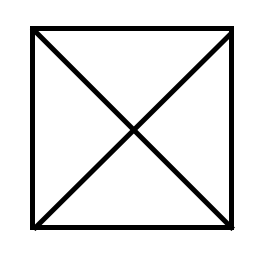
\includegraphics[scale=0.5]{Imagenes/IMG1/square.png}
\end{figure}
\end{ejemplo}
\begin{solucion}
Claramente hay 4 triángulos pequeños y cuatro triángulos grandes que se forman uniendo dos triángulos pequeños, por lo que son 8 triángulos en total. Es decir,
\[\underbrace{4}_{\text{triángulos pequeños}}+\underbrace{4}_{\text{triángulos grandes}}=8\;.\]
\end{solucion}

\begin{ejemplo}
¿cuántos cuadrados puedes encontrar en la figura \ref{cuadrado}?
\begin{figure}[h]
    \centering
    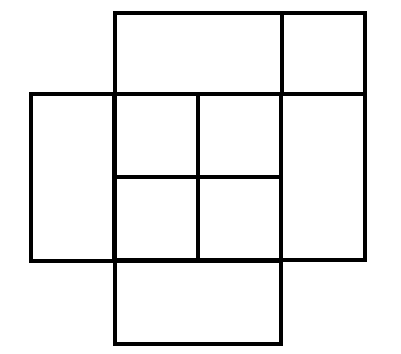
\includegraphics[scale=0.5]{Imagenes/IMG1/fig.png}
    \caption{¿Podrías identificar la cantidad de cuadrados?}
    \label{cuadrado}
\end{figure}
\end{ejemplo}

\begin{solucion}
Comencemos contando los cuadrados más grandes que son $1$, el cuadrado de $3\times 3$. Luego cuente los cuadrados de $2\times 2$, que son $5$. Luego los cuadrados de $1\times 1$ que son $5$. Solo para dejar esto más claro, el inventario resultado aplicando el principio de la suma:
\begin{itemize}
    \item $3\times 3$: $1$ cuadrado;
    \item $2\times 2$: $5$ cuadrados;
    \item $1\times 1$: $5$ cuadrados
\end{itemize}
Luego el total de cuadrados es
\[1+5+5=11\;.\]
\end{solucion}

\begin{ejemplo}
Sea $X$ el conjunto de los enteros consecutivos $\left\{16,17,\ldots,51\right\}$ y sea $Y$ el conjunto de los enteros consecutivos $\left\{70,71,\ldots,111\right\}$. ¿Cuántos enteros diferentes hay en $X$ o $Y$?
\end{ejemplo}
\begin{solucion}
Para el conjunto $X$ tenemos que $|X|=51-16+1$ números y en el conjunto $Y$ tenemos. también, que $|Y|=111-70+1=42$ números. Dado que no hay superposición entre los dos conjuntos, según el principio de la suma, hay $36 + 42 = 78$ números en $X$ o $Y$.
\end{solucion}

\section{Retroalimentación}
\begin{problema}
¿Cuántos grupos diferentes integrados por un hombre y una mujer pueden formarse con $5$ hombres y $8$ mujeres, si cierto varón se rehusa a formar pareja con dos mujeres en particular?    
\end{problema}

\begin{problema}
En un tablero de $5\times 5$, ¿de cuántas maneras posibles se pueden colocar dos fichas sin que estén ni en la misma fila ni en la misma columna?
\end{problema}

\begin{problema}
Marisol tiene un dado estándar de $6$ caras y una moneda.  ¿Cuántos resultados diferentes puede obtener tirando el dado o lanzando la moneda?
\end{problema}

\begin{problema}
    Hay $8$ tarjetas con el número $10$, $5$ tarjetas con el número $100$ y $2$ tarjetas con el número $500$. ¿Cuántas sumas distintas son posibles usando de $1$ a todas las $15$ tarjetas?
\end{problema}

\begin{problema}
    ¿Cuántos números enteros positivos de $4$ dígitos tienen $2$ o más ceros?
\end{problema}

\end{document}